\chapter{Behandelte Flussalgorithmen}

%Definition von Flussnetzwerken
\section{Flüsse in Netzwerken}

Anschaulich entsprechen Flüsse in Netzwerken der Modellierung von Transportsystemen - Anwendungsfälle sind beispielsweise Wassernetze (wobei Kapazitäten den Rohrdurchmessern entsprechen, und die Menge an geflossenem Wasser dem Fluss), Straßensysteme (Kapazität: Spurbreite, Fluss: beförderte Fahrzeuge) oder Datennetze (Kapazität: Übertragungsgeschwindigkeit, Fluss: übermittelte Datenmenge).

Als Netzwerk bezeichnet man einen gerichteten Graphen $G=\left(V, E\right)$ annotiert mit einer Kapazitätsfunktion für Kanten $u: E \rightarrow \mathbb{R}^+$ (dem \emph{upper limit}), Startknoten $s$ (der \emph{source}) und Zielknoten $t$ (\emph{target}). Insgesamt notiert man folglich ein Netzwerk als 4-Tupel $N = \left(G, u, s, t\right)$. \cite{ wiki:fluesse}

Ein Fluss in einem Netz ist definiert als eine Funktion $f: E \rightarrow \mathbb{R}^+$  (auch \emph{flow}), die für jede Kante des Graphen einen Menge an Fluss bestimmt. Ein gültiger s-t-Fluss  $f$ in einem Netzwerk muss weiterhin zwei Bedingungen erfüllen:

\begin{description}
    \item [Kapazitätskonformität] Der Fluss muss auf allen Kanten unter deren Kapazitätsgrenze liegen:
    \[\forall e \in E :f(e)\leq u(e)\]
    \item [Flusserhalt] Der Fluss ist in allen Knoten abgesehen von $s$ und $t$ Konstant, es gelangt gleich viel Fluss zum Knoten, wie ihn verlässt. Bezeichnet man die Menge an eingehenden Kanten eines Knotens als $\operatorname{\delta^-}(v)\overset{\underset{\mathrm{def}}{}}{=}\{e=(x,v) \in E \mid x \in V \}$ und die Menge an ausgehenden Kanten als $\operatorname{\delta^+}(v)\overset{\underset{\mathrm{def}}{}}{=}\{e=(v,x) \in E \mid x \in V \}$, so entspricht dies der Bedingung 
    \[\forall v\in V \setminus \{s,t\} :\sum_{e\in \operatorname{\delta^-}(v)}f(e)
=\sum_{e \in \operatorname{\delta^+}(v)}f(e)\]
\end{description}

Ein wichtiges Konzept für Flussalgorithmen ist die Konstruktion des zu einem Fluss gehörigen Residualnetzwerkes. Dieses verwendet die gleiche Knotenmenge, enthält allerdings eine neu konstruierte Kantenmenge und andere Kapazitäten. Intuitiv modelliert das Residualnetzwerk welche Änderungen des Flusses möglich sind - es enthält jede Kanten der ursprünglichen Netzwerks, falls zusätzlicher Fluss auf der Kante möglich ist, mit angepasster Kapazität. Für Kanten, die bereits Fluss tragen, werden zusätzlich Rückkanten mit Kapazität entsprechend des Flusses auf der Kante eingefügt, da es möglich wäre, diesen Fluss wieder zurückzuleiten.

\vspace{0.5cm}
\begin{minipage}[t]{0.99\textwidth}
    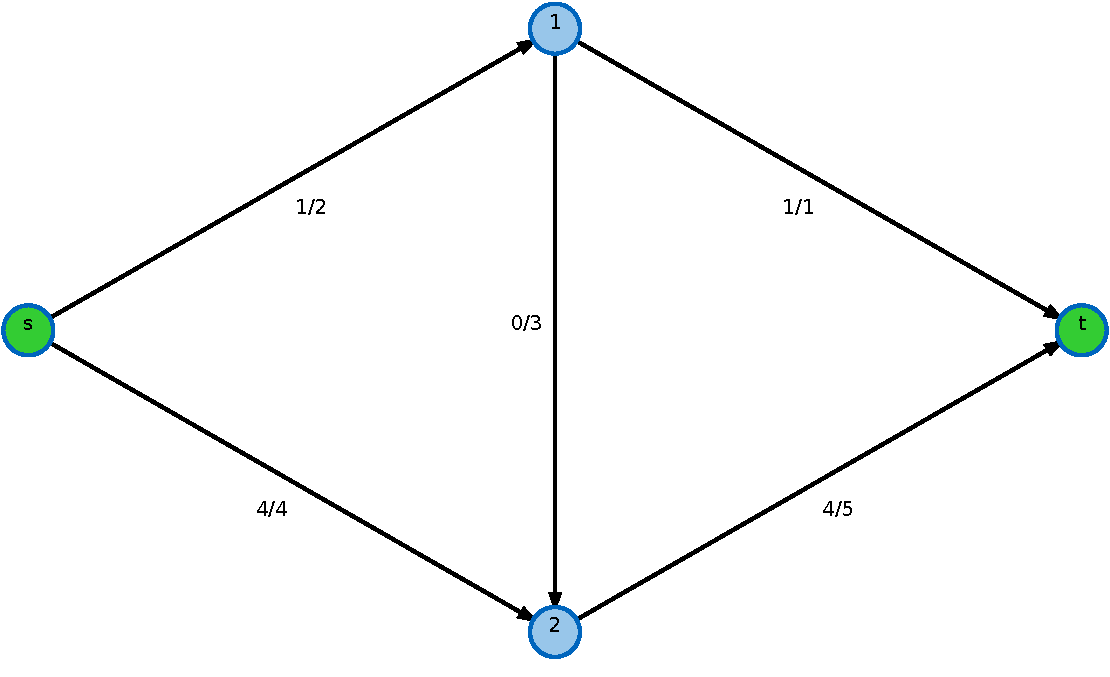
\includegraphics[width=0.8\textwidth]{img/network.pdf}
    \captionof{figure}{Ein Netzwerk mit Fluss.}
\end{minipage}
\begin{minipage}[t]{0.99\textwidth}
    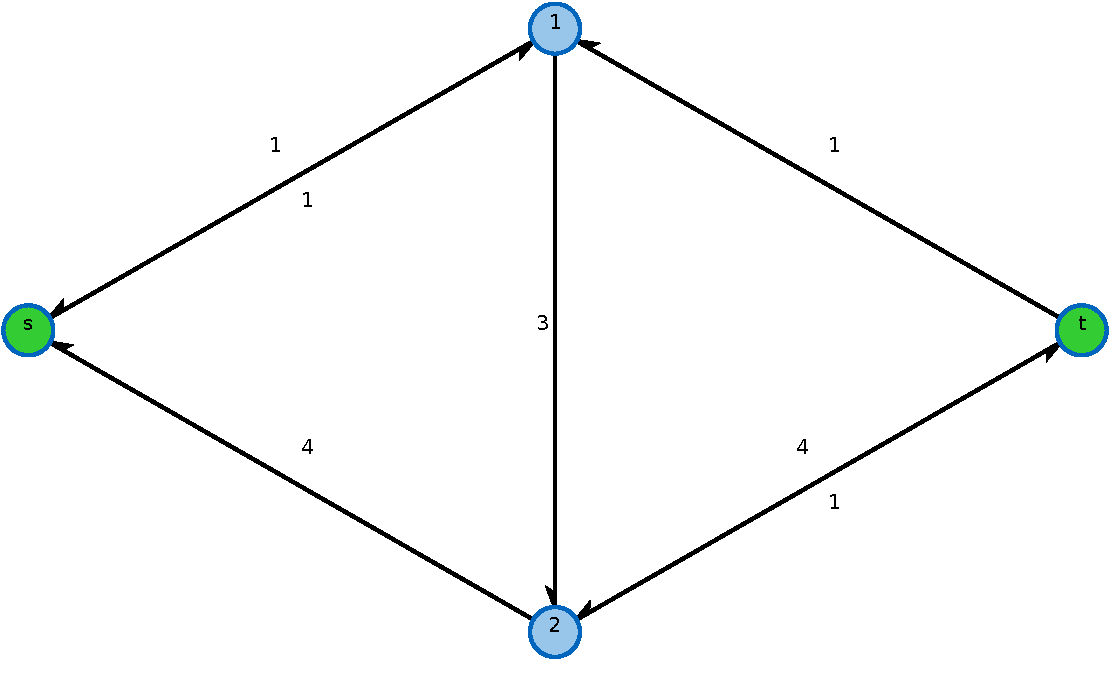
\includegraphics[width=0.8\textwidth]{img/network-residual.pdf}
    \captionof{figure}{Das zugehörige Residualnetzwerk.}
\end{minipage}

\section{Ford-Fulkerson Algorithmus}

Eine der intuitivsten Fragestellungen für ein gegebenes Netzwerk ist, wie viel Fluss gleichzeitig transportiert werden kann. Dies entspricht der Suche nach einem maximalen Fluss, das \emph{maximum flow problem}. Zur Berechnung maximaler Flüsse gibt es eine Reihe verschiedener Methoden, die sich in der Komplexität der Berechnung und Effizienz unterscheiden. Ein einfacher Algorithmus, der gleichzeitig Ausgangspunkt für eine Reihe an fortgeschritteneren Methoden bietet, ist der\emph{Ford-Fulkerson Algorithmus}. \cite{Ford-Fulkerson_algo}

Der Ford-Fulkerson Algorithmus berechnet den maximal möglichen Fluss, indem ausgehend von einem gültigen Fluss (dem Null-Fluss) wiederholt zusätzlicher Fluss durch das Netzwerk geschickt wird, ohne die Bedingungen zu verletzen. Sobald keine weiteren Änderungen mehr möglich sind ist der maximale Fluss gefunden.

Um eine gültige Änderung zu finden wird zunächst das Residualnetz des aktuellen Flusses konstruiert. In diesem wird dann ein Pfad gesucht, der Start- und Zielknoten verbindet. Entlang dieses \emph{augmentierenden Pfades} wird dann der Fluss um so viel erhöht, bis eine Kante saturiert und aus dem Residualnetz entfernt wird. Dies ist immer die Kante des Pfades mit der minimalen Residual-Kapazität. Diese Prozedur wird dann mit dem neuen Fluss wiederholt, bis kein Pfad mehr gefunden werden kann.

Die genaue Vorgehensweise für die Suche nach dem augmentierenden Pfad ist für den Ford-Fulkerson Algorithmus nicht exakt spezifiziert - sie hat allerdings starke Auswirkungen auf die Effizienz des Algorithmus. Naive Tiefensuche führt zu nichtpolynomieller Laufzeit $\mathcal{O}\left(|V|\cdot |E|\cdot u_{\max}\right)$, und auch das nur falls alle Kapazitäten ganzzahlig sind. Ein Breitensuche-Verfahren läuft dagegen schon in $\mathcal{O}(|V| \cdot |E|^2)$, diese spezielle Anwendung wird als \emph{Edmonds-Karp-Algorithmus} bezeichnet. \cite{Edmonds_karp} Eine weitere Verbesserung stellt mit einer Laufzeit von $\mathcal{O}(|V|^2 \cdot |E|)$ der \emph{Algorithmus von Dinic} dar, der nur kürzeste augmentierende Pfade verwendet. \cite{dinic70}\cite{Dinic}

\pagebreak
\begin{center}
\begin{minipage}[t]{0.65\textwidth}
    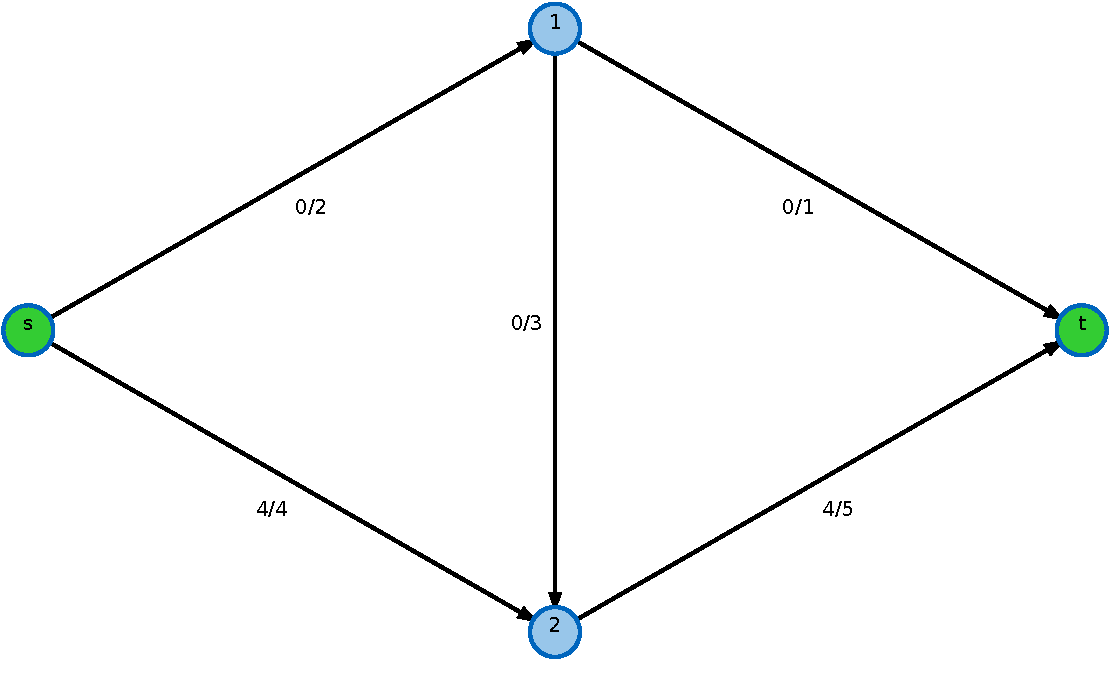
\includegraphics[width=\textwidth]{img/ford-fulkerson-1.pdf}
    \captionof{figure}{Ein initialer Fluss.}
\end{minipage}
\\
\begin{minipage}[t]{0.65\textwidth}
    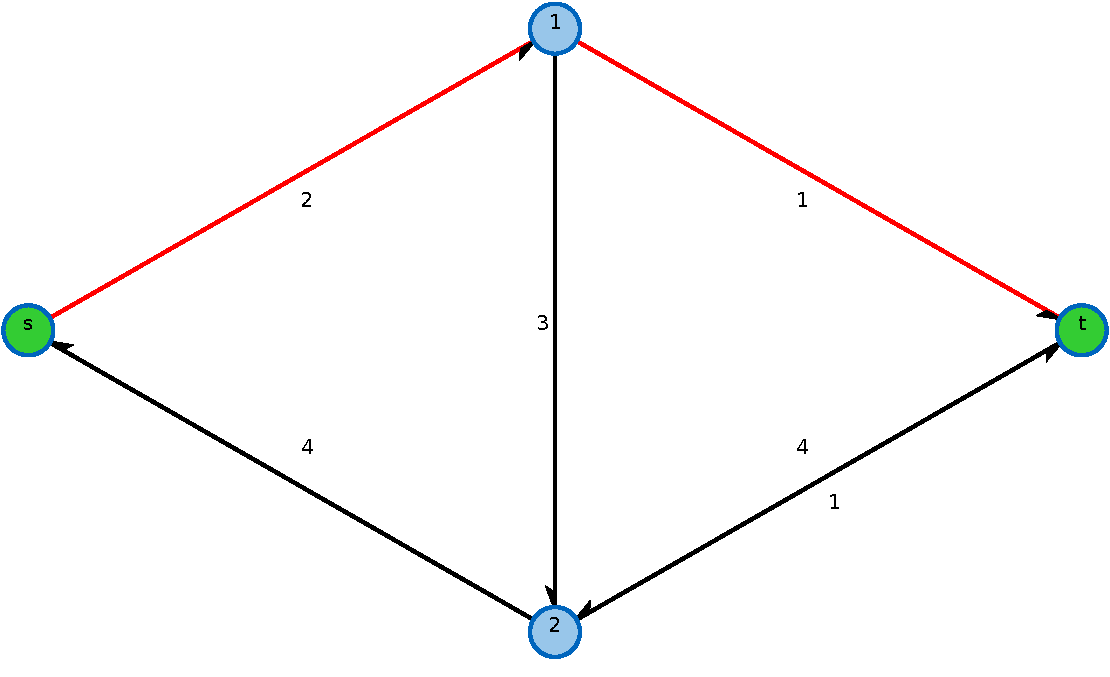
\includegraphics[width=\textwidth]{img/ford-fulkerson-2.pdf}
    \captionof{figure}{Ein augmentierender Pfad im Residualnetz.}
\end{minipage}
\\
\begin{minipage}[t]{0.65\textwidth}
    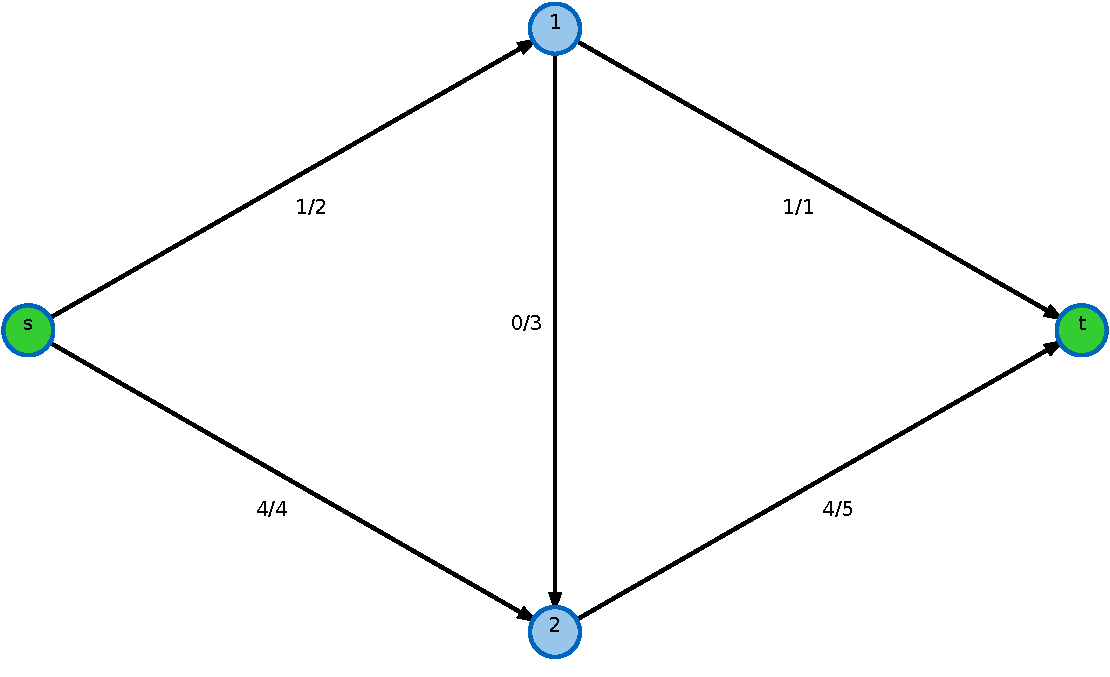
\includegraphics[width=\textwidth]{img/ford-fulkerson-3.pdf}
    \captionof{figure}{Der neue Fluss nach Modifikation.}
\end{minipage}
\end{center}

\section{Cycle Canceling Algorithmus}

Eine neue Klasse von Problemen stellt sich, sobald das Netzwerk zusätzlich mit einer Kostenfunktion auf den Kanten annotiert wird. Dies ist eine Funktion $c: E \rightarrow \mathbb{R}$ die jeder Kante zuordnet, wie teuer es ist, eine Einheit Fluss über die Kante zu transportieren. Für einen Fluss ergeben sich dann die Gesamtkosten als
\[C = \sum_{e \in E} c(e) \cdot f(e)\]

Es ergibt sich die Frage nach der günstigsten Möglichkeit, eine bestimme Menge an Fluss durch das Netzwerk zu leiten - das \emph{min-cost flow problem}. Eine übliche Variation ist zusätzlich den größtmöglichen Fluss (nach wie vor zu niedrigst möglichen Kosten) zu suchen, was man als \emph{min-cost max flow problem} bezeichnet.

Ein relativ einfacher Algorithmus zur Berechnung von Flüssen mit minimalen Kosten ist der \emph{Cycle Cancelling Algorithmus}.\cite{cycle_canceling} Der Ansatz ist dem Ford-Fulkerson Algorithmus ähnlich, da auch hier eine eine vorläufige Lösung, ein gültiger Fluss der gesuchten Gesamtmenge, iterativ verbessert wird. Dazu werden Kreise im Residualnetz gesucht, die negative Gesamtkosten besitzen. Die Umleitung von Fluss entlang eines solchen Kreises verändert den Gesamtfluss nicht, senk allerdings die Kosten. Es kann so viel Fluss umgeleitet werden, bis die Kante des Kreises mit geringster Residualkapazität aus dem Residualnetz entfernt werden muss. Diese Ablauf kann wiederholt werden, bis keine negativen Kreise mehr im Residualnetz gefunden werden.

Zur Suche nach negativen Kreisen eignet sich der \emph{Bellman-Ford Algorithmus}, ausgeführt auf dem Residualgraphen mit den Kantenkosten als Gewichtungen und ausgehend vom Zielknoten. 

Der allgemeine Cycle Canceling Algorithmus führt zu einer nichtpolynomiellen Laufzeit in $\mathcal{O}\left(|V|\cdot |E|\cdot C_{max}\right)$, da jede Iteration eine Ausführung des Bellman-Ford Algorithmus mit Laufzeit $\mathcal{O}\left(|V|\cdot |E|\right)$ erfordert und die Kosten um mindestens $1$ verringert. Eine Abwandlung mit polynomieller Laufzeit stellt das \emph{Minimum Mean Cycle Canceling Verfahren} dar.\cite{min_mean_cycle_canceling}

\pagebreak
\begin{center}
\begin{minipage}[t]{0.60\textwidth}
    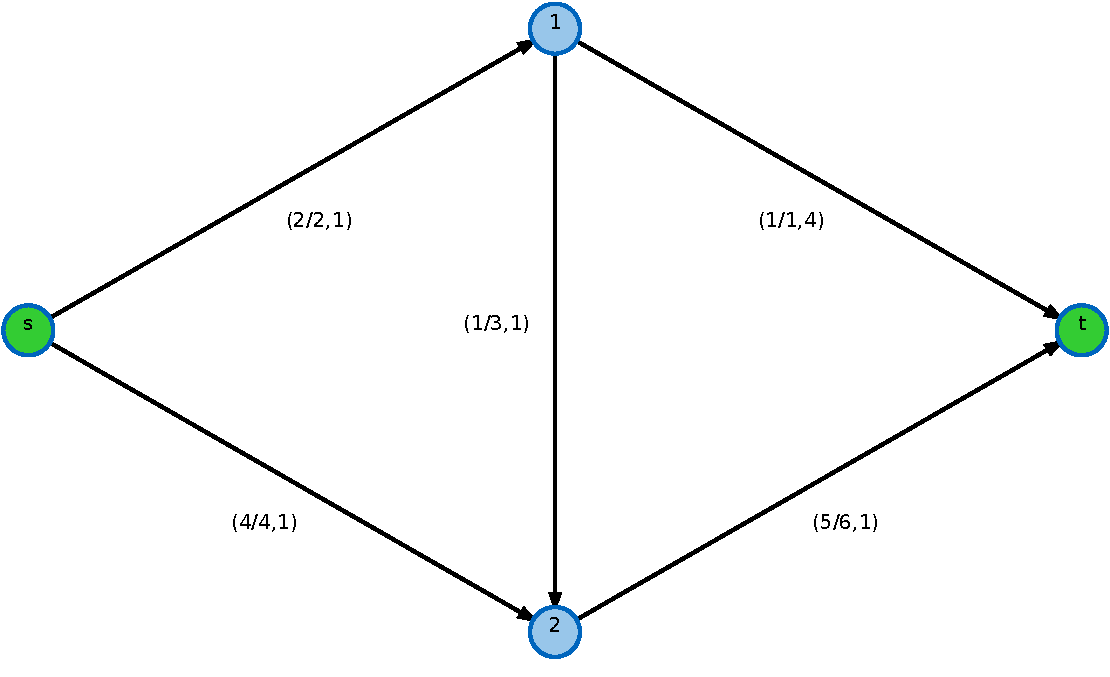
\includegraphics[width=\textwidth]{img/cycle-canceling-1.pdf}
    \captionof{figure}{Ein initialer maximaler Fluss.}
\end{minipage}
\\
\begin{minipage}[t]{0.60\textwidth}
    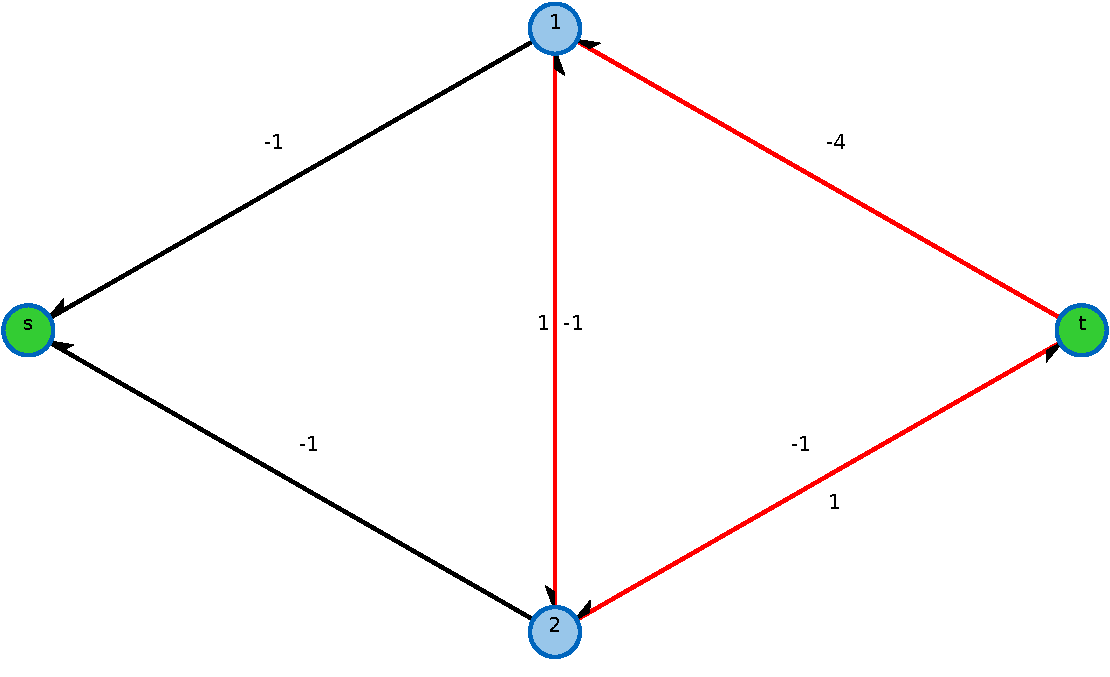
\includegraphics[width=\textwidth]{img/cycle-canceling-2.pdf}
    \captionof{figure}{Das Residualnetz enthält einen negativen Kreis.}
\end{minipage}
\\
\begin{minipage}[t]{0.60\textwidth}
    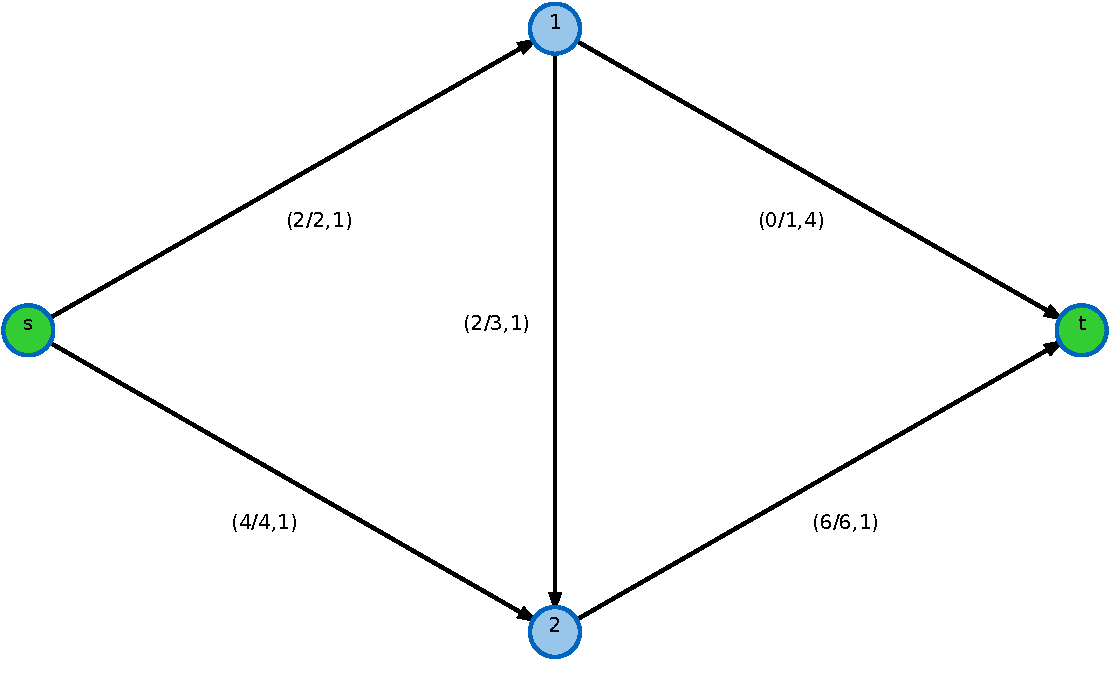
\includegraphics[width=\textwidth]{img/cycle-canceling-3.pdf}
    \captionof{figure}{Fluss nach Verschiebung entlang des negativen Kreises.}
\end{minipage}
\end{center}
